In diesem Abschnitt werden die erzielten Ergebnisse des Projekts beschrieben und kritisch bewertet. Der Fokus liegt auf der funktionalen Umsetzung, der Leistungsbewertung des Systems und einer Analyse der Stärken und Schwächen.

\subsection{Funktionale Ergebnisse}

Das Projektziel, einen voll funktionsfähigen Prototypen für einen smarten Cocktailautomaten zu entwickeln, wurde erfolgreich erreicht. Die wesentlichen funktionalen Anforderungen konnten umgesetzt werden:

\begin{itemize}
  \item \textbf{Automatisierte Cocktailzubereitung:} Die Hardware steuert präzise die Pumpen und Motoren, um Zutaten gemäß den Rezeptvorgaben abzugeben.
  \item \textbf{Mobile App:} Benutzer können über eine intuitive App Rezepte erstellen, verwalten und Bestellungen auslösen.
  \item \textbf{Backend-Integration:} Das Backend verarbeitet Bestellungen zuverlässig, synchronisiert Benutzerdaten und leitet Steuerbefehle an die Hardware weiter.
\end{itemize}

Die abschließenden Integrationstests zeigten, dass das Gesamtsystem von der Rezeptbestellung in der App bis zur Zubereitung durch die Hardware stabil funktioniert.

\subsection{Lasttestergebnisse und Analyse}

Zur Bewertung der Performance und Skalierbarkeit des Systems wurden umfassende Lasttests mit dem Tool \texttt{k6} durchgeführt. Diese Tests simulierten eine Vielzahl gleichzeitiger Benutzeranfragen, um Engpässe und Optimierungspotenziale zu identifizieren. Die wichtigsten Ergebnisse sind im Folgenden zusammengefasst.

\subsubsection*{Wichtige Metriken}
\begin{itemize}
    \item \textbf{Gesamtanfragen:} 16.506
    \item \textbf{Fehlerrate:} 0,08\% (14 fehlgeschlagene Anfragen)
    \item \textbf{Durchschnittliche Antwortzeit:} 274,48 ms
    \item \textbf{Maximale Antwortzeit:} 282.415,99 ms
    \item \textbf{90. Perzentil der Antwortzeit:} 78,66 ms
    \item \textbf{95. Perzentil der Antwortzeit:} 121,84 ms
\end{itemize}

\subsubsection*{Antwortzeiten pro Endpunkt}

Die Antwortzeiten für spezifische API-Endpunkte zeigen deutliche Unterschiede, die auf unterschiedliche Verarbeitungskomplexität hinweisen. Die wichtigsten Werte sind in Tabelle \ref{tab:response_times} dargestellt.

\begin{table}[h!]
    \centering
    \begin{tabular}{|l|c|c|c|c|}
        \hline
        \textbf{Endpunkt} & \textbf{Durchschnitt (ms)} & \textbf{Median (ms)} & \textbf{90. Perzentil (ms)} & \textbf{Max (ms)} \\
        \hline
        Registrierung & 145,60 & 102,71 & 219,24 & 1.224,99 \\
        Login & 155,91 & 102,52 & 283,80 & 1.530,32 \\
        Rezept anlegen & 136,99 & 19,10 & 42,42 & 282.282,60 \\
        Slot setzen & 1.341,94 & 23,35 & 79,70 & 282.292,87 \\
        \"Get Slots\" & 64,93 & 48,97 & 112,32 & 355,33 \\
        \"Get Favorites\" & 29,59 & 20,02 & 51,68 & 227,09 \\
        \"Create Drink\" & 588,13 & 19,39 & 52,83 & 282.275,99 \\
        \hline
    \end{tabular}
    \caption{Antwortzeiten pro Endpunkt}
    \label{tab:response_times}
\end{table}

\subsection{User-Test Ergebnisse}

Zur Evaluation der Benutzerfreundlichkeit, des Funktionsumfangs und der Stabilität der mobilen App wurden neun Personen eingeladen, die App zu testen. Sie bewerteten die App in den drei Kategorien auf einer Skala von 1 (schlecht) bis 5 (sehr gut). Die Ergebnisse sind in Tabelle \ref{tab:user_tests} und in der Visualisierung in Abbildung \ref{fig:user_tests} dargestellt.

\begin{table}[h!]
    \centering
    \begin{tabular}{|l|c|}
        \hline
        \textbf{Kategorie} & \textbf{Durchschnittliche Bewertung} \\
        \hline
        Benutzerfreundlichkeit & 4,44 \\
        Funktionsumfang & 4,22 \\
        Stabilität und Leistung & 4,88 \\
        \hline
    \end{tabular}
    \caption{Ergebnisse der Benutzerbewertungen}
    \label{tab:user_tests}
\end{table}

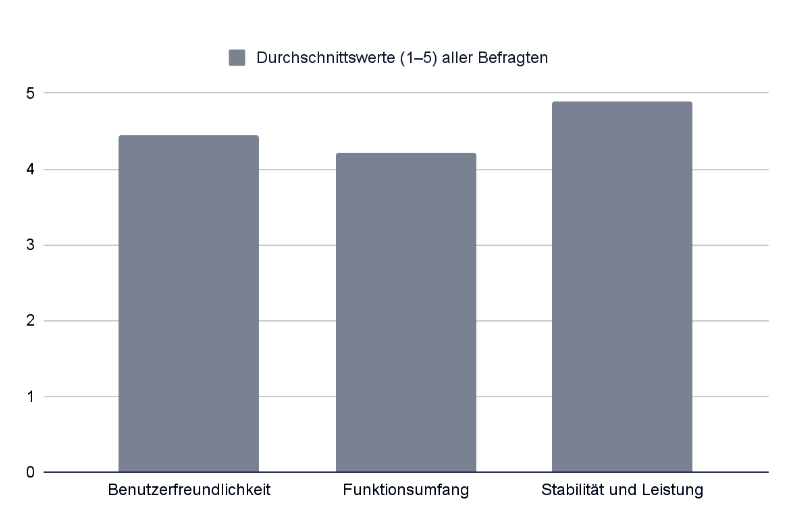
\includegraphics[width=\textwidth]{graphics/graphs/app-test.png} Balkendiagramm mit den drei Kategorien und den Durchschnittsbewertungen.

\subsection{Stärken und Schwächen}

\subsubsection*{Stärken}

Das Projekt weist folgende Stärken auf:
\begin{itemize}
  \item \textbf{Benutzerfreundlichkeit:} Die App bietet eine intuitive Benutzeroberfläche und ermöglicht eine einfache Verwaltung von Rezepten und Geräten.
  \item \textbf{Technische Umsetzung:} Die Kombination aus App, Backend und Hardware zeigt das Potenzial von IoT-Technologien in Smart-Home-Umgebungen.
  \item \textbf{Modularität:} Die Architektur des Systems ermöglicht zukünftige Erweiterungen, z. B. die Integration zusätzlicher Geräte oder neue Funktionen.
\end{itemize}

\subsubsection*{Schwächen}

Einige Schwächen des aktuellen Prototyps wurden identifiziert:
\begin{itemize}
  \item \textbf{Skalierbarkeit:} Die Verwaltung von Websocket-Verbindungen in einer containerisierten Umgebung führte bei hoher Last zu Problemen.
  \item \textbf{Fehlende Tests:} Es wurden keine umfassenden automatisierten Tests für die einzelnen Systemkomponenten implementiert.
  \item \textbf{Hardware:} Obwohl die Hardware zuverlässig arbeitet, könnten Optimierungen in der Dosiergenauigkeit und Stabilität vorgenommen werden.
\end{itemize}

\subsection{Zusammenfassung der Ergebnisse}

Das Projekt hat gezeigt, dass IoT-Technologien erfolgreich zur Automatisierung von Alltagsaufgaben eingesetzt werden können. Die entwickelten Systeme arbeiten zuverlässig und erfüllen die definierten funktionalen Anforderungen. Gleichzeitig wurden Schwächen aufgedeckt, die als Grundlage für zukünftige Optimierungen dienen können.

\subsection{Empfehlungen}

Auf Basis der Testergebnisse und identifizierten Schwächen werden folgende Maßnahmen für zukünftige Verbesserungen empfohlen:
\begin{itemize}
  \item \textbf{Optimierung der Skalierung:} Einführung eines zentralen Websocket-Servers oder konsistenter Lastverteilung, um Kommunikationsprobleme bei hoher Last zu beheben.
  \item \textbf{Automatisierte Tests:} Entwicklung und Implementierung umfassender Unit- und Integrationstests.
  \item \textbf{Hardware-Optimierungen:} Verbesserung der Dosiergenauigkeit und Integration zusätzlicher Sensorik zur Überwachung.
\end{itemize}

